\documentclass{beamer}
\beamertemplatenavigationsymbolsempty
\usecolortheme{beaver}
\setbeamertemplate{blocks}[rounded=true, shadow=true]
\setbeamertemplate{footline}[page number]
%
\usepackage[utf8]{inputenc}
\usepackage[english,russian]{babel}
\usepackage{amssymb,amsfonts,amsmath,mathtext}
\usepackage{subfig}
\usepackage[all]{xy} % xy package for diagrams
\usepackage{array}
\usepackage{multicol}% many columns in slide
\usepackage{hyperref}% urls
\usepackage{hhline}%tables
% Your figures are here:
\graphicspath{ {fig/} {../fig/} }
\documentclass{beamer}
\usepackage{graphicx}
\usepackage{amsmath}
\usepackage{hyperref}

\title{TEncDM: Понимание свойств диффузионной модели в пространстве кодировок языковых моделей}
\author{}
\date{}



\begin{document}

\frame{\titlepage}

\begin{frame}
\frametitle{Аннотация}
Представленная работа описывает Text Encoding Diffusion Model (TEncDM) — новаторский подход к моделированию текста с помощью диффузионной модели, работающей в пространстве кодировок языковой модели. TEncDM использует кодировки, которые содержат больше контекстной информации и улучшают качество предсказаний модели.
\end{frame}

\begin{frame}
\frametitle{Введение}
Авторегрессионные модели, такие как GPT-4 \cite{gpt4} и Llama 3 \cite{llama3}, демонстрируют высокое качество в генерации текста, но имеют два значительных недостатка:
\begin{itemize}
    \item Невозможность корректировать ошибки, допущенные на ранних этапах.
    \item Замедление процесса генерации для длинных последовательностей.
\end{itemize}
Диффузионные модели предлагают альтернативный метод, генерируя текст параллельно и позволяя ускорить процесс.
\end{frame}

\begin{frame}
\frametitle{Генерация с помощью диффузии}
Задача генерации текста заключается в построении текста, который удовлетворяет заданному условию, например, теме или стилю. Диффузионное моделирование предполагает преобразование случайного шума в структурированный текст.
\begin{figure}
\centering
\includegraphics[width=\textwidth]{images/diff_pic.pdf}
\end{figure}
\end{frame}

\begin{frame}
\frametitle{Генерация текста}
\begin{figure}
\centering
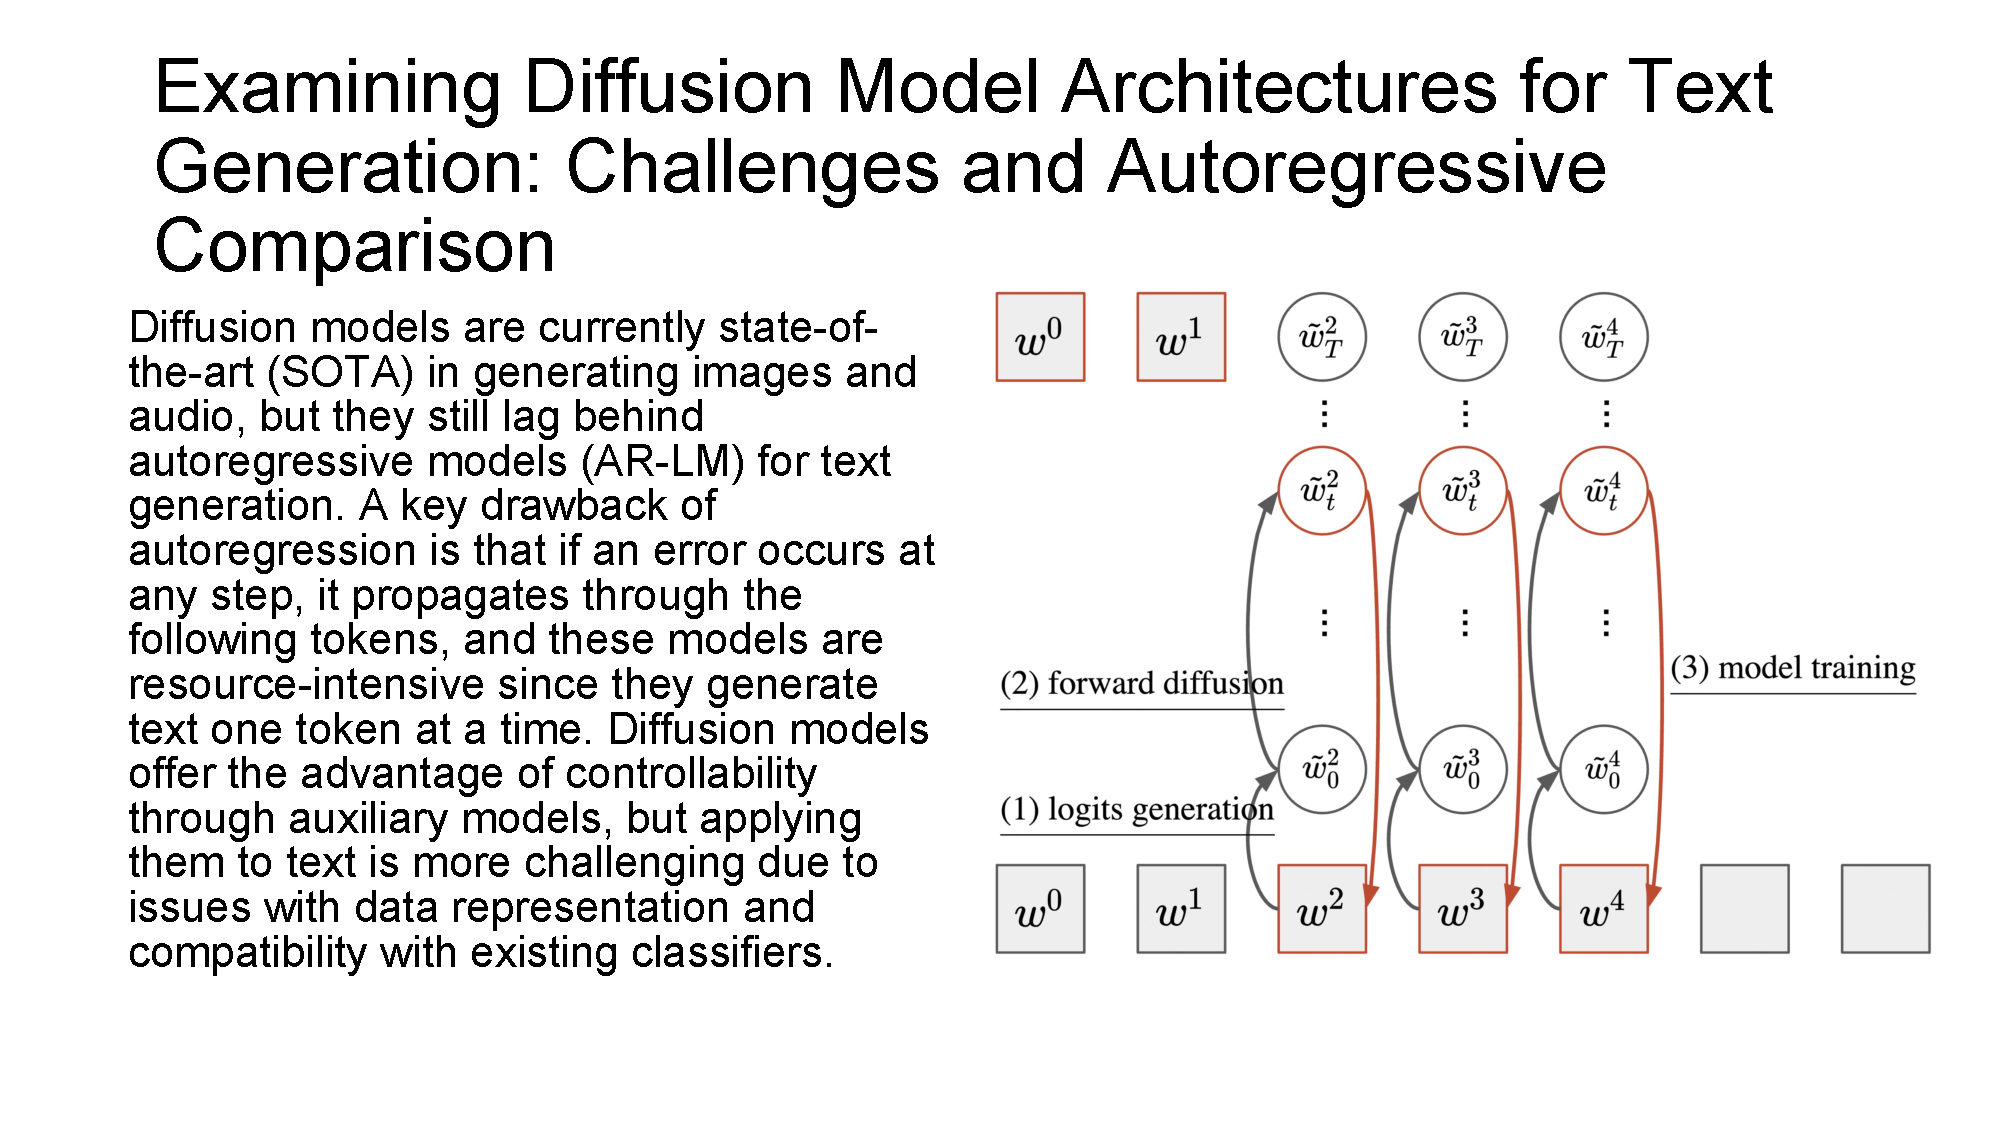
\includegraphics[width=\textwidth]{images/one_slide_talk.pdf}
\end{figure}
\end{frame}

\begin{frame}
\frametitle{Методология TEncDM}
Методология TEncDM включает несколько ключевых компонентов:
\begin{itemize}
    \item Кодировщик, использующий контекстуальные кодировки.
    \item Диффузионная модель, контролирующая добавление шума.
    \item Декодер, учитывающий контекст для каждого токена.
    \item Самоконтроль для повышения точности предсказаний.
\end{itemize}
\end{frame}

\begin{frame}
\frametitle{Обзор фреймворка}
\begin{figure}
\centering
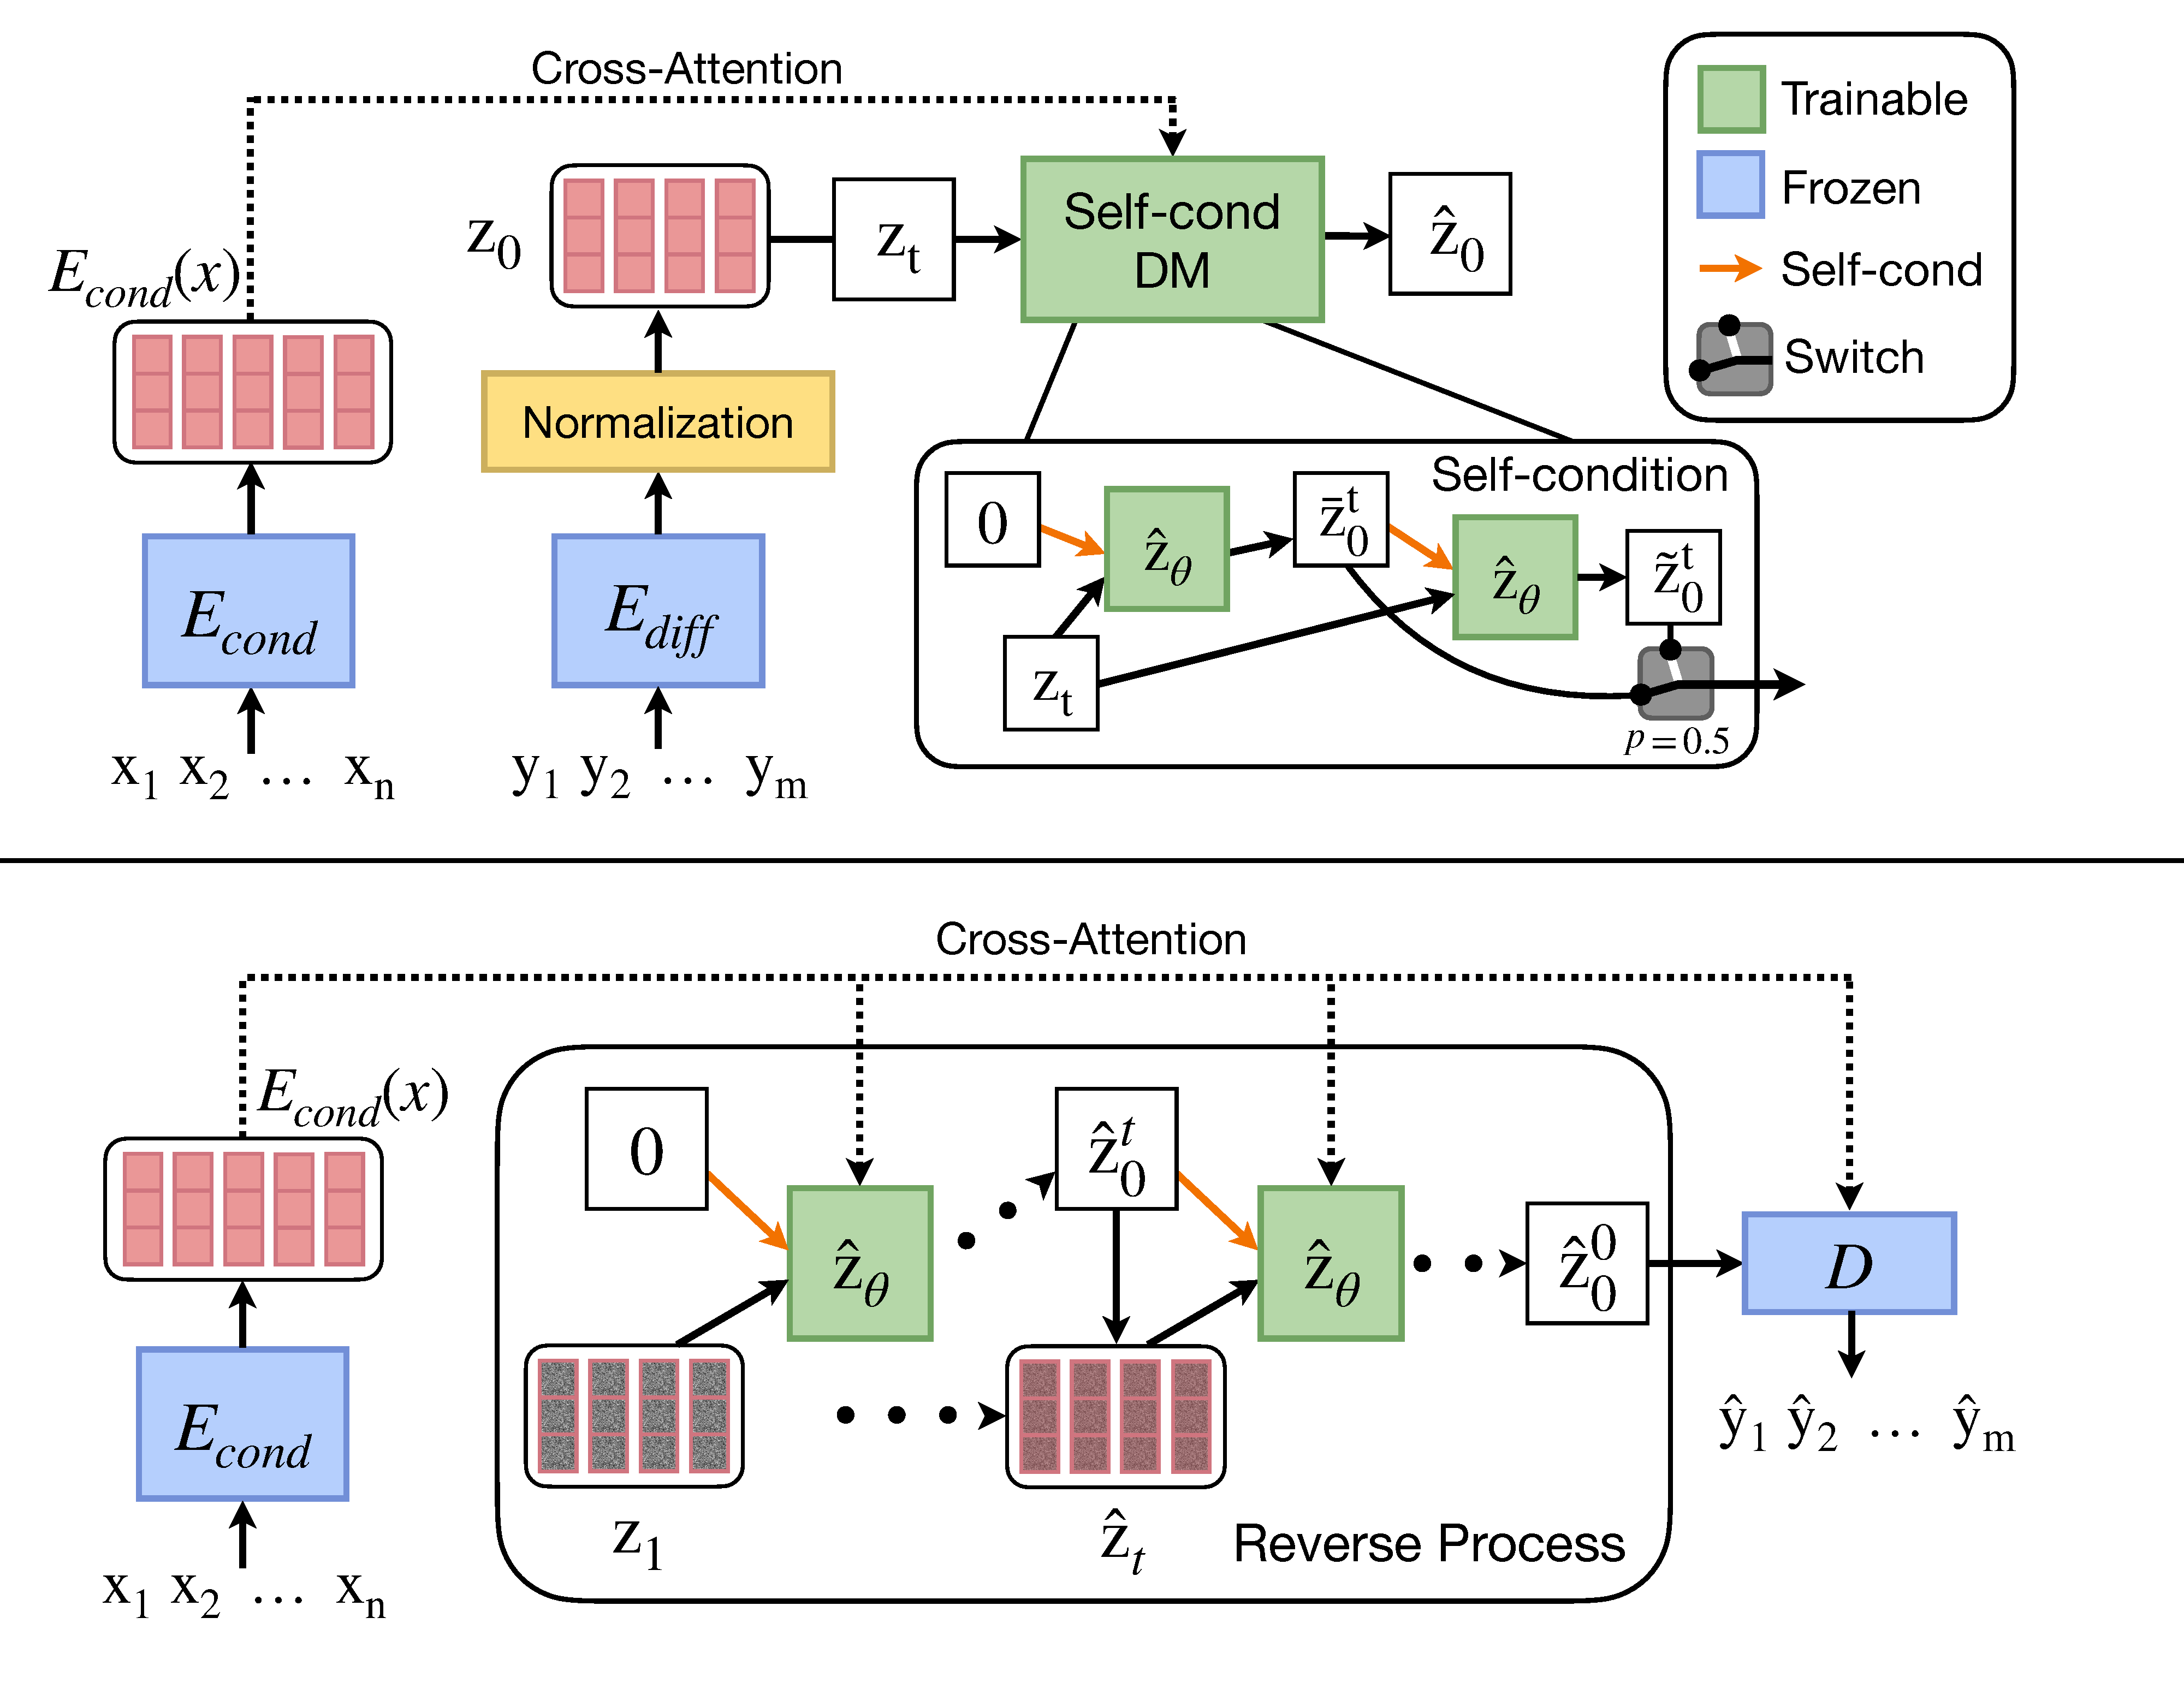
\includegraphics[width=\textwidth]{images/framework.pdf}
\caption{Обзор фреймворка для условной генерации. Вверху — процесс обучения, внизу — процесс генерации.}
\end{figure}
\end{frame}

\begin{frame}
\frametitle{Экспериментальный анализ}
Для проверки эффективности TEncDM были проведены эксперименты на задачах условной генерации текста, включая перефразирование, суммаризацию и упрощение текста. Были использованы датасеты QQP \cite{qqp} (вопросы-перефразирования), XSum \cite{xsum} (экстремальная суммаризация) и Wiki-Auto \cite{wiki_auto} (упрощение текста)
\end{frame}

\begin{frame}
\frametitle{Сравнение энкодеров}
\begin{table}
% \setlength{\tabcolsep}{3pt}
\centering
\begin{tabular}{l|llll}
\hline
\multicolumn{1}{l|}{\textbf{Encoder}}
    & \multicolumn{1}{c}{\textbf{ppl} $\downarrow$} 
    & \multicolumn{1}{c}{\textbf{mem} $\downarrow$}
    & \multicolumn{1}{c}{\textbf{div} $\uparrow$}
    & \multicolumn{1}{c}{\textbf{mauve} $\uparrow$}\\
\hline
\multicolumn{5}{c}{\textbf{ROCStories}} \\
\hline
BERT emb & $48.9_{.36}$ & $.371_{.003}$ & $.324_{.002}$ & $.600_{.016}$ \\
BERT & $29.1_{.89}$ & ${.453}_{.003}$ & ${.295}_{.002}$ & $\textbf{.762}_{.043}$ \\
RoBERTa & $\textbf{28.3}_{.33}$ & ${.443}_{.003}$ & ${.302}_{.002}$ & ${.647}_{.019}$\\
T5 & ${31.3}_{.54}$ & $.427_{.003}$ & $.312_{.004}$ & $.706_{.024}$ \\
BART & $34.1_{.52}$ & $.441_{.006}$ & $.299_{.005}$ & $.705_{.030}$\\
\hline
Source text & $21.7$ & $.365$ & $.403$ & $.876$ \\
\hline
\multicolumn{5}{c}{\textbf{Wikipedia}} \\
\hline
BERT emb & $156.1_{1.8}$ & $.263_{.004}$ & $.517_{.002}$ & $.378_{.055}$ \\
BERT & $\textbf{104.4}_{2.1}$ & $.286_{.002}$ & $.504_{.003}$ & $\textbf{.874}_{.011}$ \\
\hline
Source text & $37.3$ & $.122$ & $.615$ & $.957$ \\
\hline
\end{tabular}
\caption{Сравнение энкодеров}
\label{tab::encoders}
\end{table}
\end{frame}

\begin{frame}
\begin{table}
% \setlength{\tabcolsep}{3pt}
\centering
% \resizebox{0.49\textwidth}{!}{
\begin{tabular}{l|cccc}
\hline
\textbf{Decoder} & \textbf{ppl} $\downarrow$ & \textbf{mem} $\downarrow$ & \textbf{div} $\uparrow$ & \textbf{mauve} $\uparrow$ \\
\hline
\multicolumn{5}{c}{\textbf{ROCStories}} \\
\hline
MLP & $39.7_{3.38}$ & $.444_{.002}$ & $.297_{.004}$ & $.716_{.074}$ \\
\; + $Cor(z_0)$ & $31.2_{.33}$ & $.448_{.002}$ & $.293_{.003}$ & $.739_{.051}$ \\
Transformer & $34.2_{.29}$ & $.445_{.001}$ & $.295_{.003}$ & $.714_{.037}$ \\
\; + $Cor(z_0)$ & $\textbf{29.1}_{.89}$ & ${.453}_{.003}$ & ${.295}_{.002}$ & $\textbf{.762}_{.043}$ \\
\hline
\multicolumn{5}{c}{\textbf{Wikipedia}} \\
\hline
Transformer & $180.6_{3.2}$ & $.261_{.001}$ & $.511_{.001}$ & $.526_{.025}$ \\
\; + $Cor(z_0)$ & $\textbf{104.4}_{2.1}$ & $.286_{.002}$ & $.504_{.003}$ & $\textbf{.874}_{.011}$ \\
\hline
\end{tabular}
% }
\caption{Сравнение декодеров}
\label{tab::decoders}
\end{table}
\end{frame}

\begin{frame}
\frametitle{Заключение}
TEncDM показывает высокие результаты в задачах генерации текста и превосходит традиционные модели. Улучшение качества предсказаний достигается за счет контекстуальных кодировок и эффективного денойзинга.
\end{frame}

\begin{frame}
\frametitle{Список литературы}
\bibliographystyle{plain}
\bibliography{references}
\end{frame}

\end{document}
